  Dieses Kapitel zeigt Methoden zur Entscheidungsfindung bei einer Evaluation
  auf. Dabei werden die Methoden der gewichteten Nutzwertanalyse und des
  \ac{AHP} gezeigt. Es existieren wahrscheinlich noch weitere Ansätze, welche
  hier nicht behandelt werden.
  
  \section{Grundlagen}
  
  Es gibt verschiedene Methoden wie man bei der Auswahl einer Softwarelösung
  vorgehen kann. Um eine möglichst objektive Betrachtung zu gewährleisten, wurde
  die Methode der gewichteten \ac{NWA} gewählt, siehe \cite{Nutzwertanalyse}.
  Diese Methode stammt aus dem Bereich der quantitativen Analysemethoden der
  Eintscheidungstheorie. Um eine möglichst präzise objektive Gewichtung der
  einzelnen Faktoren zu erhalten wurde die Methode \ac{AHP} gewählt, siehe
  \cite{AnalyticHierarchyProcess}. Diese Methode stammt aus dem Bereich der
  präskriptiven Entscheidungstheorie. Der \ac{AHP} wurde von Thomas L. Saaty in
  den 70er Jahren des 20. Jahrhunderts entwickelt und im Buch ``The Analytic
  Hierarchy Process: Planning, Priority Setting, Resource
  Allocation'', siehe \cite{AnalyticHierarchyProcessBook}, veröffentlicht.
  
  \section{Gewichtete Nutzwertanalyse}
  
  Bei der gewichteten \ac{NWA} wird eine Menge von Alternativen, auf deren
  Nutzen, miteinander verglichen. Der Vergleich wird über \(n\) vergleichbare
  Kriterien geführt. Dabei werden die einzelnen Kriterien mit einem
  Erfüllungsgrad \(e_i\) bewertet. Die Skala der Erfüllungsgrade ist in der
  Tabelle \ref{tab:erfuellungsgrade} ersichtlich.
  \newline
  
  \begin{table}[ht]
    \sffamily 
    \begin{center}
      \begin{tabular}{lc}
        \toprule
        Erfüllungsgrad & Skala\\
        \midrule
        nicht erfüllt & 0\\
        schlecht & 1, 2\\
        mittel & 3 - 5\\
        gut & 6 - 8\\
        sehr gut & 9\\
        \bottomrule
      \end{tabular}
      \caption{Skala der Erfüllungsgrade}
      \label{tab:erfuellungsgrade}
    \end{center}
  \end{table}
  
  Jedes Kriterium wird durch einen Gewichtungsfaktor \(g_i\) versehen, was
  die Präferenz des Kriteriums wiederspiegelt. Dabei gilt: Die Gewichte gi
  werden so gewählt, dass ihre Summe 1 (100\%) ergibt, siehe Formel \ref{eq:gewicht}.

  \begin{equation}
    \label{eq:gewicht}
    Gewicht := \sum \limits_{i=1}^n g_i = 1
  \end{equation}

  \newpage

  Der Nutzwert ergibt sich durch die Formel \ref{eq:nutzwert}:

  \begin{equation}
    \label{eq:nutzwert}
    Nutzwert := \sum \limits_{i=1}^n e_i \cdot g_i
  \end{equation}
  
  Für jede zu evaluierende Alternative soll geprüft werden, ob eines der
  KO-Kriterien erfüllt ist, was zu einem Ausschluss der Alternative führen
  würde. Falls das nicht der Fall ist, wird der Nutzwert der Alternative
  berechnet. Diejenige Alternative mit dem grössten Nutzwert entspricht am
  meisten den Anforderungen.
  
  \subsection{Anschauliches Beispiel}
  
  Als anschauliches Beispiel sollen zwei Alternativen - Auto \(A\) und \(B\) -
  miteinander verglichen werden. Sie sollen auf deren Kriterien - Leistung,
  Aussehen und Alltagstauglichkeit - verglichen werden. In der Tabelle
  \ref{tab:beispielNwa} ist das Beispiel ersichtlich. Das Resultat zeigt, dass
  das Auto \(A\) dem Auto \(B\) gegenüber bevorzugt werden soll, da der
  Nutzwert \(5.0 > 4.7\) ist. 
  
  \begin{table}[ht]
    \sffamily 
    \begin{center}
      \begin{tabular}{lrrrrr}
        \toprule
        Kriterien & Gewichtung \(g\) & \(e_A\) & Wertigkeit \(A\) & \(e_B\)
        & Wertigkeit \(B\)\\
        \midrule
        Leistung            & 0.3 & 7 & 2.1 & 9 & 2.7 \\
        Aussehen            & 0.2 & 2 & 0.4 & 5 & 1.0 \\
        Alltagstauglichkeit & 0.5 & 5 & 2.5 & 2 & 1.0 \\
        \midrule
        \midrule
        Ergebnis            & 1.0 &   & 5.0 &   & 4.7 \\
        \bottomrule
      \end{tabular}
      \caption{Beispiel einer Nutzwertanalyse}
      \label{tab:beispielNwa}
    \end{center}
  \end{table}
 
  \section{Analytic Hierarchy Process}
  
  Der Analytic Hierarchy Process stamt aus der Feder eines Mathematikers. Aus
  diesem Grund ist das Verfahren auch einiges Anspruchsvoller als eine
  gewichtete Nutzwertanalyse. Ich gehe hier nicht auf die ganzen Details ein, da
  es den Rahmen der Diplomarbeit übersteigen würde. Totzdem soll eine grober
  Überblick über den \ac{AHP} gegeben werden.
  
  Der \ac{AHP} besteht aus drei Phasen, siehe \cite{AnalyticHierarchyProcess}: 
  
  \begin{enumerate}
    \item Sammeln der Daten
    \item Daten vergleichen und gewichten
    \item Daten verarbeiten
  \end{enumerate}
  
  \subsection{Sammeln der Daten}
  
  In der ersten Phase sollen alle Daten, die für eine Entscheidungsfindung
  erheblich sind, gesammelt werden.
  
  \begin{itemize}
    \item Zuerst soll eine konkrete Frage formuliert werden, für welche die
    beste Antwort gesucht wird.
    \item Danach sollen zu der gestellten Frage alle Kriterien  gesucht werden,
    welche die Lösung beeinflussen können.
    \item Als letztes sollen alle Alternativen gesucht werden, welche als
    mögliche Lösung infrage kommen.
  \end{itemize}
  
  \subsection{Daten vergleichen und gewichten}
  
  In der zweiten Phase folgt nun die Gegenüberstellung, Vergleich und Bewertung
  aller Kriterien beziehungsweise Alternativen in zwei Unterschritten.
  
  \begin{itemize}
    \item Jedes Kriterium wird jedem anderen gegenübergestellt und darauf
    verlgichen, was eine grössere Bedeutung in der gestellten Frage hat. Die
    Skala geht von 1 bis 9, siehe Tabelle \ref{tab:vergleichsgrade}.
    \item Für jedes Kriterium wird jede mögliche Alternativen mit jeder anderen
    gegenübergestellt und auf ihre Eignung hin untersuchen, welche Alternative
    am besten zur Erfüllung des jeweiligen Kriteriums passt. Die Skala geht von
    1 bis 9, siehe Tabelle \ref{tab:vergleichsgrade}.
  \end{itemize}
  
  \begin{table}[ht]
    \sffamily 
    \begin{center}
      \begin{tabular}{lc}
        \toprule
        Bedeutung & Skala\\
        \midrule
        gleiche Bedeutung & 1\\
        leicht grössere Bedeutung & 2 - 3\\
        viel grössere Bedeutung & 4 - 6\\
        erheblich grössere Bedeutung & 7 - 8\\
        absolut dominierend & 9\\
        \bottomrule
      \end{tabular}
      \caption{Skala der Vergleichsgrade}
      \label{tab:vergleichsgrade}
    \end{center}
  \end{table}
    
  \subsection{Daten verarbeiten}
  
  Mit einem mathematischen Modell, kann der \ac{AHP} nun eine präzise Gewichtung
  aller Kriterien errechnen. Mit der Gewichtung der Kriterien und dem Vergleich
  der Alternativen, kann der \ac{AHP} nun berechnen, welches die beste Lösung
  (Alternative) für die gestellt Frage ist. Aus dem mathematischen Modell
  heraus, kann nun ein Inkonsistenzfaktor errechnet werden, der eine Aussage
  macht, wie logisch die Bewertungen zueinander sind.
  
  Diese Berechnungen werden meistens mit der Unterstütztung einer Software
  gemacht. Als Beispiel gibt es JAHP 2.1\footnote{Für Hintergrundinformationen
  zum JAHP 2.1, siehe \cite{JAHP}}, dies ist ein Java Programm mit dem der
  gesammte Prozess des \ac{AHP} abgebildet und berechnet werden kann. Das
  Programm wird unter den Bedingungen der GNU General Public License
  vertrieben.
    
  \section{Kombination beider Methoden}
  
  Diese beiden Methoden können auch kombiniert eingesetzt werden, siehe
  \cite{AhpNwaKombination}, da der \ac{AHP} relativ komplex in der Umsetztung
  ist. Als Kombination kann die Nutzwertanalyse als Methode verwendet werden,
  und der \ac{AHP} wird für die präzise berechnung der Gewichtung einzelner
  Entscheidungskriterien verwendet. Aus der Kombination entsteht somit eine
  neue Methode, welche durch die Verständlichkeit der \ac{NWA} und der
  objektiven Gewichtung des \ac{AHP} eine plausable Evaluation ermöglicht.
  
  In der Abbildung \ref{img:ablaufEvaluation} ist der komplette Ablauf einer
  Evaluation mit der kombinierten Methode ersichtlich.
    
  \begin{figure}[ht]
    \begin{center}
      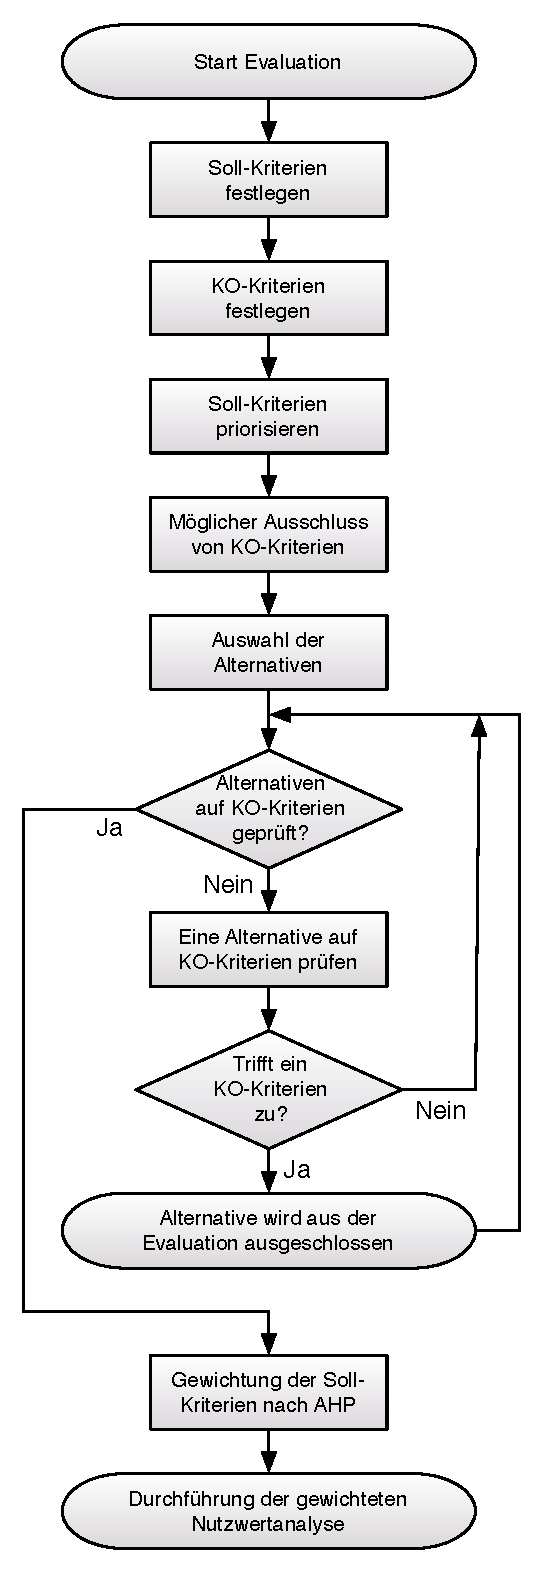
\includegraphics[width=0.47\textwidth]{./image/ablaufEvaluation.pdf}
      \caption{Ablauf einer Evaluation mit der kombinierten Methode aus
      Nutzwertanalyse und \ac{AHP}}
      \label{img:ablaufEvaluation}
    \end{center}
  \end{figure}
  
  \subsection{Verbesserung der Gewichtung}
  
  Damit die Gewichtung noch präziser bestimmt werden kann, gibt es verschiedene
  Ansätze. Zwei Ansätze möchte ich hier erläutern:
  
  \begin{itemize}
    \item Die Sensitivitätsanalyse, siehe \cite{Sensitivitaetsanalyse}.
    
    Dabei wird ein einzelner Werte in der Gewichtung gezielt verändert, und das
    Resultat wird danach geprüft. Bei der Methode des \ac{AHP} könnte zum
    Beispiel der Inkonsistenzfaktor geprüft werden, wenn dieser sich Positiv
    verändert, dann zeigt das eine Vergesserung der Gewichtung. Das Vorgehen
    wird iterativ, bis zur Unterschreitung einer definierten Schwelle des
    Inkonsistenzfaktors, fortgeführt.
    
    \item Statistische Methoden, wie der Mittelwert oder der Median, siehe
    \cite{Median} und \cite{Mittelwert}.
    
    Dabei wird der Prozess der Gewichtung von mehr als einer Person
    durchgeführt. Das Ergebniss wird aufgrund der statistischen Methoden
    normalisiert.
  \end{itemize}
  
  Diese Ansätze zur Verbesserung der Gewichtung werden im Rahmen der
  Diplomarbeit nicht durchgeführt, sollen aber bei einer anderen Anwendung nicht
  ausgeschlossen werden.
